%package list
\documentclass{article}
\usepackage[top=3cm, bottom=3cm, outer=3cm, inner=3cm]{geometry}
\usepackage{multicol}
\usepackage{graphicx}
\usepackage{url}
%\usepackage{cite}
\usepackage{hyperref}
\usepackage{array}
%\usepackage{multicol}
\newcolumntype{x}[1]{>{\centering\arraybackslash\hspace{0pt}}p{#1}}
\usepackage{natbib}
\usepackage{pdfpages}
\usepackage{multirow}
\usepackage[normalem]{ulem}
\useunder{\uline}{\ul}{}
\usepackage{svg}
\usepackage{xcolor}
\usepackage{listings}
\lstdefinestyle{ascii-tree}{
    literate={├}{|}1 {─}{--}1 {└}{+}1 
  }
\lstset{basicstyle=\ttfamily,
  showstringspaces=false,
  commentstyle=\color{red},
  keywordstyle=\color{blue}
}
%\usepackage{booktabs}
\usepackage{caption}
\usepackage{subcaption}
\usepackage{float}
\usepackage{array}

\newcolumntype{M}[1]{>{\centering\arraybackslash}m{#1}}
\newcolumntype{N}{@{}m{0pt}@{}}


%%%%%%%%%%%%%%%%%%%%%%%%%%%%%%%%%%%%%%%%%%%%%%%%%%%%%%%%%%%%%%%%%%%%%%%%%%%%
%%%%%%%%%%%%%%%%%%%%%%%%%%%%%%%%%%%%%%%%%%%%%%%%%%%%%%%%%%%%%%%%%%%%%%%%%%%%
\newcommand{\itemEmail}{vmamanian@unsa.edu.pe}
\newcommand{\itemStudent}{Victor Mamani Anahua}
\newcommand{\itemCourse}{Fundamentos de la Programación II}
\newcommand{\itemCourseCode}{20230489}
\newcommand{\itemSemester}{II}
\newcommand{\itemUniversity}{Universidad Nacional de San Agustín de Arequipa}
\newcommand{\itemFaculty}{Facultad de Ingeniería de Producción y Servicios}
\newcommand{\itemDepartment}{Departamento Académico de Ingeniería de Sistemas e Informática}
\newcommand{\itemSchool}{Escuela Profesional de Ingeniería de Sistemas}
\newcommand{\itemAcademic}{2023 - B}
\newcommand{\itemInput}{Del 22 Diciembre 2023}
\newcommand{\itemOutput}{Al 23 Diciembre 2023}
\newcommand{\itemPracticeNumber}{03}
\newcommand{\itemTheme}{Trabajo 03}
%%%%%%%%%%%%%%%%%%%%%%%%%%%%%%%%%%%%%%%%%%%%%%%%%%%%%%%%%%%%%%%%%%%%%%%%%%%%
%%%%%%%%%%%%%%%%%%%%%%%%%%%%%%%%%%%%%%%%%%%%%%%%%%%%%%%%%%%%%%%%%%%%%%%%%%%%

\usepackage[english,spanish]{babel}
\usepackage[utf8]{inputenc}
\AtBeginDocument{\selectlanguage{spanish}}
\renewcommand{\figurename}{Figura}
\renewcommand{\refname}{Referencias}
\renewcommand{\tablename}{Tabla} %esto no funciona cuando se usa babel
\AtBeginDocument{%
	\renewcommand\tablename{Tabla}
}

\usepackage{fancyhdr}
\pagestyle{fancy}
\fancyhf{}
\setlength{\headheight}{30pt}
\renewcommand{\headrulewidth}{1pt}
\renewcommand{\footrulewidth}{1pt}
\fancyhead[L]{\raisebox{-0.2\height}{
\includegraphics[width=3cm]{img/logo_episunsa.png}}}
\fancyhead[C]{\fontsize{7}{7}\selectfont	\itemUniversity \\ \itemFaculty \\ \itemDepartment \\ \itemSchool \\ \textbf{\itemCourse}}
\fancyhead[R]{\raisebox{-0.2\height}{
\includegraphics[width=1.2cm]{img/logo_abet}}}
\fancyfoot[L]{Estudiante Victor Mamani A.}
\fancyfoot[C]{\itemCourse}
\fancyfoot[R]{Página \thepage}

% para el codigo fuente
\usepackage{listings}
\usepackage{color, colortbl}
\definecolor{dkgreen}{rgb}{0,0.6,0}
\definecolor{gray}{rgb}{0.5,0.5,0.5}
\definecolor{mauve}{rgb}{0.58,0,0.82}
\definecolor{codebackground}{rgb}{0.95, 0.95, 0.92}
\definecolor{tablebackground}{rgb}{0.8, 0, 0}

\lstdefinestyle{java}{frame=tb,
	language=Java,
	showstringspaces=false,
	columns=flexible,
	basicstyle={\footnotesize\ttfamily\color[RGB]{255,255,255}},
	numberstyle=\color{mygray},
	numbers=left, 
	keywordstyle=\color{myblue},
	morekeywords={String, System},
	commentstyle=\color{mygray},
	stringstyle=\color{mygreen},
	breaklines=true,
	breakatwhitespace=true,
	tabsize=2,
	backgroundcolor= \color{codebackgroundCode},
	showspaces=false,
	showtabs=false,
	showlines=false,
}

\lstset{frame=tb,
	language=bash,
	aboveskip=3mm,
	belowskip=3mm,
	showstringspaces=false,
	columns=flexible,
	basicstyle={\small\ttfamily},
	numbers=none,
	numberstyle=\tiny\color{gray},
	keywordstyle=\color{blue},
	commentstyle=\color{dkgreen},
	stringstyle=\color{mauve},
	breaklines=true,
	breakatwhitespace=true,
	tabsize=3,
	backgroundcolor= \color{codebackground},
}

\begin{document}
	
	\vspace*{10px}
	
	\begin{center}	
		\fontsize{17}{17} \textbf{ Informe de Trabajo \itemPracticeNumber}
	\end{center}
	\centerline{\textbf{\Large Tema: \itemTheme}}
	%\vspace*{0.5cm}	

	\begin{flushright}
		\begin{tabular}{|M{2.5cm}|N|}
			\hline 
			\rowcolor{tablebackground}
			\color{white} \textbf{Nota}  \\
			\hline 
			     \\[30pt]
			\hline 			
		\end{tabular}
	\end{flushright}	

	\begin{table}[H]
		\begin{tabular}{|x{4.7cm}|x{4.8cm}|x{4.8cm}|}
			\hline 
			\rowcolor{tablebackground}
			\color{white} \textbf{Estudiante} & \color{white}\textbf{Escuela}  & \color{white}\textbf{Asignatura}   \\
			\hline 
			{\itemStudent \par \itemEmail} & \itemSchool & {\itemCourse \par Semestre: \itemSemester \par Código: \itemCourseCode}     \\
			\hline 			
		\end{tabular}
	\end{table}		
	
	\begin{table}[H]
		\begin{tabular}{|x{4.7cm}|x{4.8cm}|x{4.8cm}|}
			\hline 
			\rowcolor{tablebackground}
			\color{white}\textbf{Trabajo} & \color{white}\textbf{Tema}  & \color{white}\textbf{Duración}   \\
			\hline 
			\itemPracticeNumber & \itemTheme & 04 horas   \\
			\hline 
		\end{tabular}
	\end{table}
	
	\begin{table}[H]
		\begin{tabular}{|x{4.7cm}|x{4.8cm}|x{4.8cm}|}
			\hline 
			\rowcolor{tablebackground}
			\color{white}\textbf{Semestre académico} & \color{white}\textbf{Fecha de inicio}  & \color{white}\textbf{Fecha de entrega}   \\
			\hline 
			\itemAcademic & \itemInput &  \itemOutput  \\
			\hline 
		\end{tabular}
	\end{table}
	
	\section{Tarea}
	\begin{itemize}		
        \item Crear una clase base denominada Punto que conste de las coordenadas x e y. A
		partir de esta clase, definir una clase denominada Circulo que tenga las coordenadas del
		centro y un atributo denominado radio. Entre las funciones miembro de la primera clase,
		deberá existir una función distancia() que devuelva la distancia entre dos puntos, donde:
		Distancia = ((x2 – x1) 2 + (y2 – y1) 2) 1/2
        \item Utilizando la clase construida en el ejercicio 01, obtener una clase derivada
		Cilindro derivada de Circulo. La clase Cilindro deberá tener una función miembro que calcule
		la superficie de dicho cilindro. La fórmula que calcula la superficie del cilindro es S = 2r(l + r)
		donde r es el radio del cilindro y l es la longitud.
        \item Caso de estudio especial: herencia múltiple. Es un tipo de herencia en la que una
		clase hereda el estado (estructura) y el comportamiento de más de una clase base. (hay
		herencia múltiple cuando una clase hereda de más de una clase). Java no permite la herencia
		múltiple, pero se puede conseguir la implementación de la herencia múltiple usando
		interfaces. Implemente el siguiente diagrama de clases UML y consiga pruebas válidas.
		\end{itemize}

	\section{Equipos, materiales y temas utilizados}
	\begin{itemize}
		\item Sistema Operativo Ubuntu GNU Linux 23 lunar 64 bits Kernell 6.2.v
		\item Visual Studio Code.
		\item VIM 9.0.
		\item OpenJDK 64-Bits 19.0.7.
		\item Git 2.39.2.
		\item Cuenta en GitHub con el correo institucional.
		\item Programación Orientada a Objetos.
		\item Actividades del Trabajo03.	
	\end{itemize}
	
	\section{URL de Repositorio Github}
	\begin{itemize}
		\item URL del Repositorio GitHub para clonar o recuperar.
		\item \url{https://github.com/VictorMA18/fp2-23b.git}
		\item URL para el Trabajo03 en el Repositorio GitHub.
		\item \url{https://github.com/VictorMA18/fp2-23b/tree/main/Fase02/Trabajo03}
	\end{itemize}
	
	\section{Actividades del Trabajo03}

	\subsection{Ejercicio1}
	\begin{itemize}	
		\item En el primer programa creamos la clase Punto tiene atributos x e y, un constructor para asignar coordenadas, y un método para calcular la distancia entre dos puntos. La clase Circulo hereda de Punto e incluye un radio. En el programa principal (Ejercicio1), se crean instancias de Punto y Circulo, se calcula la distancia entre dos puntos y se imprime la información del círculo. La implementación demuestra la relación de herencia entre las clases
	\end{itemize}	
	\begin{lstlisting}[language=java,caption={Las lineas de codigos del metodo creado:}][H]
		class Punto{
			protected double x;
			protected double y;
			public Punto(double x, double y){ //Creamos un constructor para asiganar valores a los atributos de la clase Punto el cual nos podra asignar puntos como para un centro de nuestra figura o de un punti cualquiera
				this.x = x;
				this.y = y;
			}
			public double distancia(Punto fin){ //Metodo que nos permite ver la distancia entre puntos o hallar la distancia de un centro de nuestra figura hacia un punto 
				double distanciax = this.x - fin.x;
				double distanciay = this.y - fin.y;
				double distanciaresultante = (distanciax * distanciax) + (distanciay * distanciay);
				return Math.sqrt(distanciaresultante);
			}
			public String toString(){ //Cree este metodo para que nos puedra mostrar los puntos que estamos calculando
				return "(" + this.x + " , " + this.y + ")";
			}
		}
		class Circulo extends Punto{
			protected double radio;
			public Circulo(double x, double y, double radio){ //Creamos este constructor el cual nos va a establecer las coordenadas que necesitamos como su centro y asignamos el valor del radio de este
				super(x,y); //Llamamos al constructor de la clase Punto ,la cual seria nuestro centro del circulo de lo cual heredamos de la clase Punto 
				this.radio = radio; 
			}
			public String toString(){ //Cree este metodo para que nos puedra mostrar las propiedades de este como su centro y su radio
				return ("El centro del circulo es : " + "(" + this.x + " , " + this.y + ")" + " y su radio es : " + this.radio);
			}
		}
		class Ejercicio1{
			public static void main(String[] args) {
				Punto puntoinicial = new Punto(0, 0);
				Punto puntofinal = new Punto(3, 4);
				double distanciaentrepuntos = puntoinicial.distancia(puntofinal);
				System.out.println("El punto inicial: " + puntoinicial.toString() + " y el punto final: " + puntofinal.toString());
				System.out.println("La distancia entre estos es: " + distanciaentrepuntos);
				Circulo circulo = new Circulo(2, 1, 5);
				System.out.println(circulo.toString());
			}
		}
	\end{lstlisting}
	\begin{figure}[H]
		\centering
		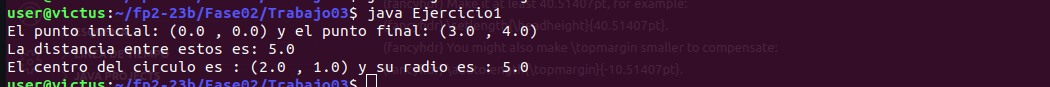
\includegraphics[width=1.0\textwidth,keepaspectratio]{img/Captura.png}
		%\includesvg{img/automata.svg}
		%\label{img:mot2}
		%\caption{Product backlog.}
	\end{figure}
	\subsection{Ejercicio2}
	\begin{itemize}	
		\item En el segundo programa creamos la clase Cilindro, que extiende la clase Circulo. La clase Cilindro representa un cilindro tridimensional con un centro, un radio y una altura. Su constructor llama al constructor de la clase Circulo para establecer el centro y el radio y asigna la altura adicional. La clase incluye un método para calcular la superficie del cilindro y un método toString() que devuelve una representación en cadena que incluye las propiedades del cilindro. En el programa principal (Ejercicio2), se crea una instancia de Cilindro con coordenadas, radio y altura específicos, se calcula la superficie y se imprime la información del cilindro junto con su superficie. 
	\end{itemize}	
	\begin{lstlisting}[language=java,caption={Las lineas de codigos del metodo creado:}][H]
		class Cilindro extends Circulo {
			protected double altura;
			public Cilindro (double x , double y , double radio , double altura){ //Creamos este constructor el cual nos va a establecer las coordenadas que necesitamos como su centro , radio y la longitud de este cilindro
				super(x, y, radio); //llamamos al constructor del cual heredamos esta clase que es Circulo lo cual nos ayudara en nuestra clase Cilindro para tener un centro y un radio definido
				this.altura = altura; //asignamos la altura 
			}
			public double superficie(){
				double superficiecilindro = ((2 * (this.radio)) * (this.altura + this.radio)); 
				return superficiecilindro;
			}
			public String toString(){ //Cree este metodo el cual me ayuda a de
				return ("El centro del cilindro es : " + "(" + this.x + " , " + this.y + ")" + " , su radio es : " + this.radio + " y su altura es: " + this.altura);
			}
		}
		class Ejercicio2 {
			public static void main(String[] args) {
				Cilindro cilindro = new Cilindro(2, 4, 5, 10);
				double superficiecilindro = cilindro.superficie();
				System.out.println(cilindro.toString());
				System.out.println("La superficie de este cilindro es : " + superficiecilindro);
			}
		}
	\end{lstlisting}
	\begin{figure}[H]
		\centering
		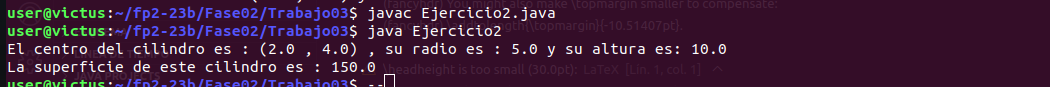
\includegraphics[width=1.0\textwidth,keepaspectratio]{img/Captura2.png}
		%\includesvg{img/automata.svg}
		%\label{img:mot2}
		%\caption{Product backlog.}
	\end{figure}
	\subsection{Ejercicio3}
	\begin{itemize}	
		\item En el tercer programa creamos dos interfaces, Barco y Avion, cada una con un método específico (zarpar y planear, respectivamente). Luego, se implementa la herencia múltiple a través de la clase Hidroavion, que implementa ambas interfaces. En el programa principal (Ejercicio3), se crea un objeto Hidroavion, y se llaman a sus métodos zarpar y planear, demostrando la implementación exitosa de ambas interfaces. Además, se utilizan referencias de tipo Barco y Avion para hacer referencia al mismo objeto Hidroavion
	\end{itemize}	
	\begin{lstlisting}[language=java,caption={Las lineas de codigos del metodo creado:}][H]
		interface Barco {
			void zarpar();
		}
		interface Avion{
			void planear();
		}
		class Hidroavion implements Barco, Avion{ //Creamos las interfaces como una herdacion multiple la cual Hidroavion tiene esta condicion donde este puede aplicar metodos de las interfaces creadas
			public void zarpar(){ //Metodo de la interfaz Barco
				System.out.println("El Hidroavion esta implementando el metodo zarpar de la interfaz Barco");
			} 
			public void planear() {
				System.out.println("El Hidroavion esta implementando el metodo planear de la interfaz Avion");
			} 
		}
		class Ejercicio3 {
			public static void main(String[] args) {
				Hidroavion hidroavion = new Hidroavion();
				hidroavion.zarpar();
				hidroavion.planear();//Comprobando la heredacion multiple por interfaces la cual creamos a un objeto hidroavion que usara metodos de las interfaces de la cual se hereda
				Barco barco = hidroavion; //La referencia de tipo Barco para hacer referencia a una instancia de Hidroavion.
				Avion avion = hidroavion; //La referencia de tipo Avion para hacer referencia a una instancia de Hidroavion.
				barco.zarpar();
				avion.planear();
			}
		}
	\end{lstlisting}
	\begin{figure}[H]
		\centering
		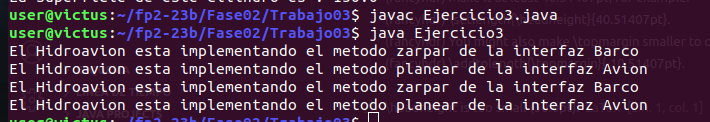
\includegraphics[width=1.0\textwidth,keepaspectratio]{img/Captura3.png}
		%\includesvg{img/automata.svg}
		%\label{img:mot2}
		%\caption{Product backlog.}
	\end{figure}
	\subsection{Estructura de Trabajo03}
	\begin{itemize}	
		\item El contenido que se entrega en este Trabajo03 es el siguiente:
	\end{itemize}
	\begin{lstlisting}[style=ascii-tree]
	/Trabajo03	
	├── Avion.class
	├── Barco.class
	├── Cilindro.class
	├── Circulo.class
	├── Ejercicio1.class
	├── Ejercicio1.java
	├── Ejercicio2.class
	├── Ejercicio2.java
	├── Ejercicio3.class
	├── Ejercicio3.java
	├── Hidroavion.class
	├── Latex
	│   ├── img
	│   │   ├── Captura2.png
	│   │   ├── Captura3.png
	│   │   ├── Captura.png
	│   │   ├── logo_abet.png
	│   │   ├── logo_episunsa.png
	│   │   └── logo_unsa.jpg
	│   ├── Informe.aux
	│   ├── Informe.fdb_latexmk
	│   ├── Informe.fls
	│   ├── Informe.log
	│   ├── Informe.out
	│   ├── Informe.pdf
	│   ├── Informe.synctex.gz
	│   └── Informe.tex
	└── Punto.class
	
	\end{lstlisting}    
	\section{\textcolor{red}{Rúbricas}}
	
	\subsection{\textcolor{red}{Entregable Informe}}
	\begin{table}[H]
		\caption{Tipo de Informe}
		\setlength{\tabcolsep}{0.5em} % for the horizontal padding
		{\renewcommand{\arraystretch}{1.5}% for the vertical padding
		\begin{tabular}{|p{3cm}|p{12cm}|}
			\hline
			\multicolumn{2}{|c|}{\textbf{\textcolor{red}{Informe}}}  \\
			\hline 
			\textbf{\textcolor{red}{Latex}} & \textcolor{blue}{El informe está en formato PDF desde Latex,  con un formato limpio (buena presentación) y facil de leer.}   \\ 
			\hline 
			
			
		\end{tabular}
	}
	\end{table}
	
	\clearpage
	
	\subsection{\textcolor{red}{Rúbrica para el contenido del Informe y demostración}}
	\begin{itemize}			
		\item El alumno debe marcar o dejar en blanco en celdas de la columna \textbf{Checklist} si cumplio con el ítem correspondiente.
		\item Si un alumno supera la fecha de entrega,  su calificación será sobre la nota mínima aprobada, siempre y cuando cumpla con todos lo items.
		\item El alumno debe autocalificarse en la columna \textbf{Estudiante} de acuerdo a la siguiente tabla:
	
		\begin{table}[ht]
			\caption{Niveles de desempeño}
			\begin{center}
			\begin{tabular}{ccccc}
    			\hline
    			 & \multicolumn{4}{c}{Nivel}\\
    			\cline{1-5}
    			\textbf{Puntos} & Insatisfactorio 25\%& En Proceso 50\% & Satisfactorio 75\% & Sobresaliente 100\%\\
    			\textbf{2.0}&0.5&1.0&1.5&2.0\\
    			\textbf{4.0}&1.0&2.0&3.0&4.0\\
    		\hline
			\end{tabular}
		\end{center}
	\end{table}	
	
	\end{itemize}
	
	\begin{table}[H]
		\caption{Rúbrica para contenido del Informe y demostración}
		\setlength{\tabcolsep}{0.5em} % for the horizontal padding
		{\renewcommand{\arraystretch}{1.5}% for the vertical padding
		%\begin{center}
		\begin{tabular}{|p{2.7cm}|p{7cm}|x{1.3cm}|p{1.2cm}|p{1.5cm}|p{1.1cm}|}
			\hline
    		\multicolumn{2}{|c|}{Contenido y demostración} & Puntos & Checklist & Estudiante & Profesor\\
			\hline
			\textbf{1. GitHub} & Hay enlace URL activo del directorio para el trabajo hacia su repositorio GitHub con código fuente terminado y fácil de revisar. &2 &X &2 & \\ 
			\hline
			\textbf{2. Commits} &  Hay capturas de pantalla de los commits más importantes con sus explicaciones detalladas. (El profesor puede preguntar para refrendar calificación). &4 &X &4 & \\ 
			\hline 
			\textbf{3. Código fuente} &  Hay porciones de código fuente importantes con numeración y explicaciones detalladas de sus funciones. &2 &X &2 & \\ 
			\hline 
			\textbf{4. Ejecución} & Se incluyen ejecuciones/pruebas del código fuente  explicadas gradualmente. &2 &X &2 & \\ 
			\hline			
			\textbf{5. Pregunta} & Se responde con completitud a la pregunta formulada en la tarea.  (El profesor puede preguntar para refrendar calificación).  &2 &X &2 & \\ 
			\hline	
			\textbf{6. Fechas} & Las fechas de modificación del código fuente estan dentro de los plazos de fecha de entrega establecidos. &2 &X &2 & \\ 
			\hline 
			\textbf{7. Ortografía} & El documento no muestra errores ortográficos. &2 &X &2 & \\ 
			\hline 
			\textbf{8. Madurez} & El Informe muestra de manera general una evolución de la madurez del código fuente,  explicaciones puntuales pero precisas y un acabado impecable.   (El profesor puede preguntar para refrendar calificación).  &4 &X &2 & \\ 
			\hline
			\multicolumn{2}{|c|}{\textbf{Total}} &20 & &18 & \\ 
			\hline
		\end{tabular}
		%\end{center}
		%\label{tab:multicol}
		}
	\end{table}
	
\clearpage

\section{Referencias}
	
%\clearpage
%\bibliographystyle{apalike}
%\bibliographystyle{IEEEtranN}
%\bibliography{bibliography}
			
\end{document}